\documentclass[11pt]{article}

    \usepackage[breakable]{tcolorbox}
    \usepackage{parskip} % Stop auto-indenting (to mimic markdown behaviour)
    

    % Basic figure setup, for now with no caption control since it's done
    % automatically by Pandoc (which extracts ![](path) syntax from Markdown).
    \usepackage{graphicx}
    % Keep aspect ratio if custom image width or height is specified
    \setkeys{Gin}{keepaspectratio}
    % Maintain compatibility with old templates. Remove in nbconvert 6.0
    \let\Oldincludegraphics\includegraphics
    % Ensure that by default, figures have no caption (until we provide a
    % proper Figure object with a Caption API and a way to capture that
    % in the conversion process - todo).
    \usepackage{caption}
    \DeclareCaptionFormat{nocaption}{}
    \captionsetup{format=nocaption,aboveskip=0pt,belowskip=0pt}

    \usepackage{float}
    \floatplacement{figure}{H} % forces figures to be placed at the correct location
    \usepackage{xcolor} % Allow colors to be defined
    \usepackage{enumerate} % Needed for markdown enumerations to work
    \usepackage{geometry} % Used to adjust the document margins
    \usepackage{amsmath} % Equations
    \usepackage{amssymb} % Equations
    \usepackage{textcomp} % defines textquotesingle
    % Hack from http://tex.stackexchange.com/a/47451/13684:
    \AtBeginDocument{%
        \def\PYZsq{\textquotesingle}% Upright quotes in Pygmentized code
    }
    \usepackage{upquote} % Upright quotes for verbatim code
    \usepackage{eurosym} % defines \euro

    \usepackage{iftex}
    \ifPDFTeX
        \usepackage[T1]{fontenc}
        \IfFileExists{alphabeta.sty}{
              \usepackage{alphabeta}
          }{
              \usepackage[mathletters]{ucs}
              \usepackage[utf8x]{inputenc}
          }
    \else
        \usepackage{fontspec}
        \usepackage{unicode-math}
    \fi

    \usepackage{fancyvrb} % verbatim replacement that allows latex
    \usepackage{grffile} % extends the file name processing of package graphics
                         % to support a larger range
    \makeatletter % fix for old versions of grffile with XeLaTeX
    \@ifpackagelater{grffile}{2019/11/01}
    {
      % Do nothing on new versions
    }
    {
      \def\Gread@@xetex#1{%
        \IfFileExists{"\Gin@base".bb}%
        {\Gread@eps{\Gin@base.bb}}%
        {\Gread@@xetex@aux#1}%
      }
    }
    \makeatother
    \usepackage[Export]{adjustbox} % Used to constrain images to a maximum size
    \adjustboxset{max size={0.9\linewidth}{0.9\paperheight}}

    % The hyperref package gives us a pdf with properly built
    % internal navigation ('pdf bookmarks' for the table of contents,
    % internal cross-reference links, web links for URLs, etc.)
    \usepackage{hyperref}
    % The default LaTeX title has an obnoxious amount of whitespace. By default,
    % titling removes some of it. It also provides customization options.
    \usepackage{titling}
    \usepackage{longtable} % longtable support required by pandoc >1.10
    \usepackage{booktabs}  % table support for pandoc > 1.12.2
    \usepackage{array}     % table support for pandoc >= 2.11.3
    \usepackage{calc}      % table minipage width calculation for pandoc >= 2.11.1
    \usepackage[inline]{enumitem} % IRkernel/repr support (it uses the enumerate* environment)
    \usepackage[normalem]{ulem} % ulem is needed to support strikethroughs (\sout)
                                % normalem makes italics be italics, not underlines
    \usepackage{soul}      % strikethrough (\st) support for pandoc >= 3.0.0
    \usepackage{mathrsfs}
    

    
    % Colors for the hyperref package
    \definecolor{urlcolor}{rgb}{0,.145,.698}
    \definecolor{linkcolor}{rgb}{.71,0.21,0.01}
    \definecolor{citecolor}{rgb}{.12,.54,.11}

    % ANSI colors
    \definecolor{ansi-black}{HTML}{3E424D}
    \definecolor{ansi-black-intense}{HTML}{282C36}
    \definecolor{ansi-red}{HTML}{E75C58}
    \definecolor{ansi-red-intense}{HTML}{B22B31}
    \definecolor{ansi-green}{HTML}{00A250}
    \definecolor{ansi-green-intense}{HTML}{007427}
    \definecolor{ansi-yellow}{HTML}{DDB62B}
    \definecolor{ansi-yellow-intense}{HTML}{B27D12}
    \definecolor{ansi-blue}{HTML}{208FFB}
    \definecolor{ansi-blue-intense}{HTML}{0065CA}
    \definecolor{ansi-magenta}{HTML}{D160C4}
    \definecolor{ansi-magenta-intense}{HTML}{A03196}
    \definecolor{ansi-cyan}{HTML}{60C6C8}
    \definecolor{ansi-cyan-intense}{HTML}{258F8F}
    \definecolor{ansi-white}{HTML}{C5C1B4}
    \definecolor{ansi-white-intense}{HTML}{A1A6B2}
    \definecolor{ansi-default-inverse-fg}{HTML}{FFFFFF}
    \definecolor{ansi-default-inverse-bg}{HTML}{000000}

    % common color for the border for error outputs.
    \definecolor{outerrorbackground}{HTML}{FFDFDF}

    % commands and environments needed by pandoc snippets
    % extracted from the output of `pandoc -s`
    \providecommand{\tightlist}{%
      \setlength{\itemsep}{0pt}\setlength{\parskip}{0pt}}
    \DefineVerbatimEnvironment{Highlighting}{Verbatim}{commandchars=\\\{\}}
    % Add ',fontsize=\small' for more characters per line
    \newenvironment{Shaded}{}{}
    \newcommand{\KeywordTok}[1]{\textcolor[rgb]{0.00,0.44,0.13}{\textbf{{#1}}}}
    \newcommand{\DataTypeTok}[1]{\textcolor[rgb]{0.56,0.13,0.00}{{#1}}}
    \newcommand{\DecValTok}[1]{\textcolor[rgb]{0.25,0.63,0.44}{{#1}}}
    \newcommand{\BaseNTok}[1]{\textcolor[rgb]{0.25,0.63,0.44}{{#1}}}
    \newcommand{\FloatTok}[1]{\textcolor[rgb]{0.25,0.63,0.44}{{#1}}}
    \newcommand{\CharTok}[1]{\textcolor[rgb]{0.25,0.44,0.63}{{#1}}}
    \newcommand{\StringTok}[1]{\textcolor[rgb]{0.25,0.44,0.63}{{#1}}}
    \newcommand{\CommentTok}[1]{\textcolor[rgb]{0.38,0.63,0.69}{\textit{{#1}}}}
    \newcommand{\OtherTok}[1]{\textcolor[rgb]{0.00,0.44,0.13}{{#1}}}
    \newcommand{\AlertTok}[1]{\textcolor[rgb]{1.00,0.00,0.00}{\textbf{{#1}}}}
    \newcommand{\FunctionTok}[1]{\textcolor[rgb]{0.02,0.16,0.49}{{#1}}}
    \newcommand{\RegionMarkerTok}[1]{{#1}}
    \newcommand{\ErrorTok}[1]{\textcolor[rgb]{1.00,0.00,0.00}{\textbf{{#1}}}}
    \newcommand{\NormalTok}[1]{{#1}}

    % Additional commands for more recent versions of Pandoc
    \newcommand{\ConstantTok}[1]{\textcolor[rgb]{0.53,0.00,0.00}{{#1}}}
    \newcommand{\SpecialCharTok}[1]{\textcolor[rgb]{0.25,0.44,0.63}{{#1}}}
    \newcommand{\VerbatimStringTok}[1]{\textcolor[rgb]{0.25,0.44,0.63}{{#1}}}
    \newcommand{\SpecialStringTok}[1]{\textcolor[rgb]{0.73,0.40,0.53}{{#1}}}
    \newcommand{\ImportTok}[1]{{#1}}
    \newcommand{\DocumentationTok}[1]{\textcolor[rgb]{0.73,0.13,0.13}{\textit{{#1}}}}
    \newcommand{\AnnotationTok}[1]{\textcolor[rgb]{0.38,0.63,0.69}{\textbf{\textit{{#1}}}}}
    \newcommand{\CommentVarTok}[1]{\textcolor[rgb]{0.38,0.63,0.69}{\textbf{\textit{{#1}}}}}
    \newcommand{\VariableTok}[1]{\textcolor[rgb]{0.10,0.09,0.49}{{#1}}}
    \newcommand{\ControlFlowTok}[1]{\textcolor[rgb]{0.00,0.44,0.13}{\textbf{{#1}}}}
    \newcommand{\OperatorTok}[1]{\textcolor[rgb]{0.40,0.40,0.40}{{#1}}}
    \newcommand{\BuiltInTok}[1]{{#1}}
    \newcommand{\ExtensionTok}[1]{{#1}}
    \newcommand{\PreprocessorTok}[1]{\textcolor[rgb]{0.74,0.48,0.00}{{#1}}}
    \newcommand{\AttributeTok}[1]{\textcolor[rgb]{0.49,0.56,0.16}{{#1}}}
    \newcommand{\InformationTok}[1]{\textcolor[rgb]{0.38,0.63,0.69}{\textbf{\textit{{#1}}}}}
    \newcommand{\WarningTok}[1]{\textcolor[rgb]{0.38,0.63,0.69}{\textbf{\textit{{#1}}}}}
    \makeatletter
    \newsavebox\pandoc@box
    \newcommand*\pandocbounded[1]{%
      \sbox\pandoc@box{#1}%
      % scaling factors for width and height
      \Gscale@div\@tempa\textheight{\dimexpr\ht\pandoc@box+\dp\pandoc@box\relax}%
      \Gscale@div\@tempb\linewidth{\wd\pandoc@box}%
      % select the smaller of both
      \ifdim\@tempb\p@<\@tempa\p@
        \let\@tempa\@tempb
      \fi
      % scaling accordingly (\@tempa < 1)
      \ifdim\@tempa\p@<\p@
        \scalebox{\@tempa}{\usebox\pandoc@box}%
      % scaling not needed, use as it is
      \else
        \usebox{\pandoc@box}%
      \fi
    }
    \makeatother

    % Define a nice break command that doesn't care if a line doesn't already
    % exist.
    \def\br{\hspace*{\fill} \\* }
    % Math Jax compatibility definitions
    \def\gt{>}
    \def\lt{<}
    \let\Oldtex\TeX
    \let\Oldlatex\LaTeX
    \renewcommand{\TeX}{\textrm{\Oldtex}}
    \renewcommand{\LaTeX}{\textrm{\Oldlatex}}
    % Document parameters
    % Document title
    \title{04\_notes}
    
    
    
    
    
    
    
% Pygments definitions
\makeatletter
\def\PY@reset{\let\PY@it=\relax \let\PY@bf=\relax%
    \let\PY@ul=\relax \let\PY@tc=\relax%
    \let\PY@bc=\relax \let\PY@ff=\relax}
\def\PY@tok#1{\csname PY@tok@#1\endcsname}
\def\PY@toks#1+{\ifx\relax#1\empty\else%
    \PY@tok{#1}\expandafter\PY@toks\fi}
\def\PY@do#1{\PY@bc{\PY@tc{\PY@ul{%
    \PY@it{\PY@bf{\PY@ff{#1}}}}}}}
\def\PY#1#2{\PY@reset\PY@toks#1+\relax+\PY@do{#2}}

\@namedef{PY@tok@w}{\def\PY@tc##1{\textcolor[rgb]{0.73,0.73,0.73}{##1}}}
\@namedef{PY@tok@c}{\let\PY@it=\textit\def\PY@tc##1{\textcolor[rgb]{0.24,0.48,0.48}{##1}}}
\@namedef{PY@tok@cp}{\def\PY@tc##1{\textcolor[rgb]{0.61,0.40,0.00}{##1}}}
\@namedef{PY@tok@k}{\let\PY@bf=\textbf\def\PY@tc##1{\textcolor[rgb]{0.00,0.50,0.00}{##1}}}
\@namedef{PY@tok@kp}{\def\PY@tc##1{\textcolor[rgb]{0.00,0.50,0.00}{##1}}}
\@namedef{PY@tok@kt}{\def\PY@tc##1{\textcolor[rgb]{0.69,0.00,0.25}{##1}}}
\@namedef{PY@tok@o}{\def\PY@tc##1{\textcolor[rgb]{0.40,0.40,0.40}{##1}}}
\@namedef{PY@tok@ow}{\let\PY@bf=\textbf\def\PY@tc##1{\textcolor[rgb]{0.67,0.13,1.00}{##1}}}
\@namedef{PY@tok@nb}{\def\PY@tc##1{\textcolor[rgb]{0.00,0.50,0.00}{##1}}}
\@namedef{PY@tok@nf}{\def\PY@tc##1{\textcolor[rgb]{0.00,0.00,1.00}{##1}}}
\@namedef{PY@tok@nc}{\let\PY@bf=\textbf\def\PY@tc##1{\textcolor[rgb]{0.00,0.00,1.00}{##1}}}
\@namedef{PY@tok@nn}{\let\PY@bf=\textbf\def\PY@tc##1{\textcolor[rgb]{0.00,0.00,1.00}{##1}}}
\@namedef{PY@tok@ne}{\let\PY@bf=\textbf\def\PY@tc##1{\textcolor[rgb]{0.80,0.25,0.22}{##1}}}
\@namedef{PY@tok@nv}{\def\PY@tc##1{\textcolor[rgb]{0.10,0.09,0.49}{##1}}}
\@namedef{PY@tok@no}{\def\PY@tc##1{\textcolor[rgb]{0.53,0.00,0.00}{##1}}}
\@namedef{PY@tok@nl}{\def\PY@tc##1{\textcolor[rgb]{0.46,0.46,0.00}{##1}}}
\@namedef{PY@tok@ni}{\let\PY@bf=\textbf\def\PY@tc##1{\textcolor[rgb]{0.44,0.44,0.44}{##1}}}
\@namedef{PY@tok@na}{\def\PY@tc##1{\textcolor[rgb]{0.41,0.47,0.13}{##1}}}
\@namedef{PY@tok@nt}{\let\PY@bf=\textbf\def\PY@tc##1{\textcolor[rgb]{0.00,0.50,0.00}{##1}}}
\@namedef{PY@tok@nd}{\def\PY@tc##1{\textcolor[rgb]{0.67,0.13,1.00}{##1}}}
\@namedef{PY@tok@s}{\def\PY@tc##1{\textcolor[rgb]{0.73,0.13,0.13}{##1}}}
\@namedef{PY@tok@sd}{\let\PY@it=\textit\def\PY@tc##1{\textcolor[rgb]{0.73,0.13,0.13}{##1}}}
\@namedef{PY@tok@si}{\let\PY@bf=\textbf\def\PY@tc##1{\textcolor[rgb]{0.64,0.35,0.47}{##1}}}
\@namedef{PY@tok@se}{\let\PY@bf=\textbf\def\PY@tc##1{\textcolor[rgb]{0.67,0.36,0.12}{##1}}}
\@namedef{PY@tok@sr}{\def\PY@tc##1{\textcolor[rgb]{0.64,0.35,0.47}{##1}}}
\@namedef{PY@tok@ss}{\def\PY@tc##1{\textcolor[rgb]{0.10,0.09,0.49}{##1}}}
\@namedef{PY@tok@sx}{\def\PY@tc##1{\textcolor[rgb]{0.00,0.50,0.00}{##1}}}
\@namedef{PY@tok@m}{\def\PY@tc##1{\textcolor[rgb]{0.40,0.40,0.40}{##1}}}
\@namedef{PY@tok@gh}{\let\PY@bf=\textbf\def\PY@tc##1{\textcolor[rgb]{0.00,0.00,0.50}{##1}}}
\@namedef{PY@tok@gu}{\let\PY@bf=\textbf\def\PY@tc##1{\textcolor[rgb]{0.50,0.00,0.50}{##1}}}
\@namedef{PY@tok@gd}{\def\PY@tc##1{\textcolor[rgb]{0.63,0.00,0.00}{##1}}}
\@namedef{PY@tok@gi}{\def\PY@tc##1{\textcolor[rgb]{0.00,0.52,0.00}{##1}}}
\@namedef{PY@tok@gr}{\def\PY@tc##1{\textcolor[rgb]{0.89,0.00,0.00}{##1}}}
\@namedef{PY@tok@ge}{\let\PY@it=\textit}
\@namedef{PY@tok@gs}{\let\PY@bf=\textbf}
\@namedef{PY@tok@ges}{\let\PY@bf=\textbf\let\PY@it=\textit}
\@namedef{PY@tok@gp}{\let\PY@bf=\textbf\def\PY@tc##1{\textcolor[rgb]{0.00,0.00,0.50}{##1}}}
\@namedef{PY@tok@go}{\def\PY@tc##1{\textcolor[rgb]{0.44,0.44,0.44}{##1}}}
\@namedef{PY@tok@gt}{\def\PY@tc##1{\textcolor[rgb]{0.00,0.27,0.87}{##1}}}
\@namedef{PY@tok@err}{\def\PY@bc##1{{\setlength{\fboxsep}{\string -\fboxrule}\fcolorbox[rgb]{1.00,0.00,0.00}{1,1,1}{\strut ##1}}}}
\@namedef{PY@tok@kc}{\let\PY@bf=\textbf\def\PY@tc##1{\textcolor[rgb]{0.00,0.50,0.00}{##1}}}
\@namedef{PY@tok@kd}{\let\PY@bf=\textbf\def\PY@tc##1{\textcolor[rgb]{0.00,0.50,0.00}{##1}}}
\@namedef{PY@tok@kn}{\let\PY@bf=\textbf\def\PY@tc##1{\textcolor[rgb]{0.00,0.50,0.00}{##1}}}
\@namedef{PY@tok@kr}{\let\PY@bf=\textbf\def\PY@tc##1{\textcolor[rgb]{0.00,0.50,0.00}{##1}}}
\@namedef{PY@tok@bp}{\def\PY@tc##1{\textcolor[rgb]{0.00,0.50,0.00}{##1}}}
\@namedef{PY@tok@fm}{\def\PY@tc##1{\textcolor[rgb]{0.00,0.00,1.00}{##1}}}
\@namedef{PY@tok@vc}{\def\PY@tc##1{\textcolor[rgb]{0.10,0.09,0.49}{##1}}}
\@namedef{PY@tok@vg}{\def\PY@tc##1{\textcolor[rgb]{0.10,0.09,0.49}{##1}}}
\@namedef{PY@tok@vi}{\def\PY@tc##1{\textcolor[rgb]{0.10,0.09,0.49}{##1}}}
\@namedef{PY@tok@vm}{\def\PY@tc##1{\textcolor[rgb]{0.10,0.09,0.49}{##1}}}
\@namedef{PY@tok@sa}{\def\PY@tc##1{\textcolor[rgb]{0.73,0.13,0.13}{##1}}}
\@namedef{PY@tok@sb}{\def\PY@tc##1{\textcolor[rgb]{0.73,0.13,0.13}{##1}}}
\@namedef{PY@tok@sc}{\def\PY@tc##1{\textcolor[rgb]{0.73,0.13,0.13}{##1}}}
\@namedef{PY@tok@dl}{\def\PY@tc##1{\textcolor[rgb]{0.73,0.13,0.13}{##1}}}
\@namedef{PY@tok@s2}{\def\PY@tc##1{\textcolor[rgb]{0.73,0.13,0.13}{##1}}}
\@namedef{PY@tok@sh}{\def\PY@tc##1{\textcolor[rgb]{0.73,0.13,0.13}{##1}}}
\@namedef{PY@tok@s1}{\def\PY@tc##1{\textcolor[rgb]{0.73,0.13,0.13}{##1}}}
\@namedef{PY@tok@mb}{\def\PY@tc##1{\textcolor[rgb]{0.40,0.40,0.40}{##1}}}
\@namedef{PY@tok@mf}{\def\PY@tc##1{\textcolor[rgb]{0.40,0.40,0.40}{##1}}}
\@namedef{PY@tok@mh}{\def\PY@tc##1{\textcolor[rgb]{0.40,0.40,0.40}{##1}}}
\@namedef{PY@tok@mi}{\def\PY@tc##1{\textcolor[rgb]{0.40,0.40,0.40}{##1}}}
\@namedef{PY@tok@il}{\def\PY@tc##1{\textcolor[rgb]{0.40,0.40,0.40}{##1}}}
\@namedef{PY@tok@mo}{\def\PY@tc##1{\textcolor[rgb]{0.40,0.40,0.40}{##1}}}
\@namedef{PY@tok@ch}{\let\PY@it=\textit\def\PY@tc##1{\textcolor[rgb]{0.24,0.48,0.48}{##1}}}
\@namedef{PY@tok@cm}{\let\PY@it=\textit\def\PY@tc##1{\textcolor[rgb]{0.24,0.48,0.48}{##1}}}
\@namedef{PY@tok@cpf}{\let\PY@it=\textit\def\PY@tc##1{\textcolor[rgb]{0.24,0.48,0.48}{##1}}}
\@namedef{PY@tok@c1}{\let\PY@it=\textit\def\PY@tc##1{\textcolor[rgb]{0.24,0.48,0.48}{##1}}}
\@namedef{PY@tok@cs}{\let\PY@it=\textit\def\PY@tc##1{\textcolor[rgb]{0.24,0.48,0.48}{##1}}}

\def\PYZbs{\char`\\}
\def\PYZus{\char`\_}
\def\PYZob{\char`\{}
\def\PYZcb{\char`\}}
\def\PYZca{\char`\^}
\def\PYZam{\char`\&}
\def\PYZlt{\char`\<}
\def\PYZgt{\char`\>}
\def\PYZsh{\char`\#}
\def\PYZpc{\char`\%}
\def\PYZdl{\char`\$}
\def\PYZhy{\char`\-}
\def\PYZsq{\char`\'}
\def\PYZdq{\char`\"}
\def\PYZti{\char`\~}
% for compatibility with earlier versions
\def\PYZat{@}
\def\PYZlb{[}
\def\PYZrb{]}
\makeatother


    % For linebreaks inside Verbatim environment from package fancyvrb.
    \makeatletter
        \newbox\Wrappedcontinuationbox
        \newbox\Wrappedvisiblespacebox
        \newcommand*\Wrappedvisiblespace {\textcolor{red}{\textvisiblespace}}
        \newcommand*\Wrappedcontinuationsymbol {\textcolor{red}{\llap{\tiny$\m@th\hookrightarrow$}}}
        \newcommand*\Wrappedcontinuationindent {3ex }
        \newcommand*\Wrappedafterbreak {\kern\Wrappedcontinuationindent\copy\Wrappedcontinuationbox}
        % Take advantage of the already applied Pygments mark-up to insert
        % potential linebreaks for TeX processing.
        %        {, <, #, %, $, ' and ": go to next line.
        %        _, }, ^, &, >, - and ~: stay at end of broken line.
        % Use of \textquotesingle for straight quote.
        \newcommand*\Wrappedbreaksatspecials {%
            \def\PYGZus{\discretionary{\char`\_}{\Wrappedafterbreak}{\char`\_}}%
            \def\PYGZob{\discretionary{}{\Wrappedafterbreak\char`\{}{\char`\{}}%
            \def\PYGZcb{\discretionary{\char`\}}{\Wrappedafterbreak}{\char`\}}}%
            \def\PYGZca{\discretionary{\char`\^}{\Wrappedafterbreak}{\char`\^}}%
            \def\PYGZam{\discretionary{\char`\&}{\Wrappedafterbreak}{\char`\&}}%
            \def\PYGZlt{\discretionary{}{\Wrappedafterbreak\char`\<}{\char`\<}}%
            \def\PYGZgt{\discretionary{\char`\>}{\Wrappedafterbreak}{\char`\>}}%
            \def\PYGZsh{\discretionary{}{\Wrappedafterbreak\char`\#}{\char`\#}}%
            \def\PYGZpc{\discretionary{}{\Wrappedafterbreak\char`\%}{\char`\%}}%
            \def\PYGZdl{\discretionary{}{\Wrappedafterbreak\char`\$}{\char`\$}}%
            \def\PYGZhy{\discretionary{\char`\-}{\Wrappedafterbreak}{\char`\-}}%
            \def\PYGZsq{\discretionary{}{\Wrappedafterbreak\textquotesingle}{\textquotesingle}}%
            \def\PYGZdq{\discretionary{}{\Wrappedafterbreak\char`\"}{\char`\"}}%
            \def\PYGZti{\discretionary{\char`\~}{\Wrappedafterbreak}{\char`\~}}%
        }
        % Some characters . , ; ? ! / are not pygmentized.
        % This macro makes them "active" and they will insert potential linebreaks
        \newcommand*\Wrappedbreaksatpunct {%
            \lccode`\~`\.\lowercase{\def~}{\discretionary{\hbox{\char`\.}}{\Wrappedafterbreak}{\hbox{\char`\.}}}%
            \lccode`\~`\,\lowercase{\def~}{\discretionary{\hbox{\char`\,}}{\Wrappedafterbreak}{\hbox{\char`\,}}}%
            \lccode`\~`\;\lowercase{\def~}{\discretionary{\hbox{\char`\;}}{\Wrappedafterbreak}{\hbox{\char`\;}}}%
            \lccode`\~`\:\lowercase{\def~}{\discretionary{\hbox{\char`\:}}{\Wrappedafterbreak}{\hbox{\char`\:}}}%
            \lccode`\~`\?\lowercase{\def~}{\discretionary{\hbox{\char`\?}}{\Wrappedafterbreak}{\hbox{\char`\?}}}%
            \lccode`\~`\!\lowercase{\def~}{\discretionary{\hbox{\char`\!}}{\Wrappedafterbreak}{\hbox{\char`\!}}}%
            \lccode`\~`\/\lowercase{\def~}{\discretionary{\hbox{\char`\/}}{\Wrappedafterbreak}{\hbox{\char`\/}}}%
            \catcode`\.\active
            \catcode`\,\active
            \catcode`\;\active
            \catcode`\:\active
            \catcode`\?\active
            \catcode`\!\active
            \catcode`\/\active
            \lccode`\~`\~
        }
    \makeatother

    \let\OriginalVerbatim=\Verbatim
    \makeatletter
    \renewcommand{\Verbatim}[1][1]{%
        %\parskip\z@skip
        \sbox\Wrappedcontinuationbox {\Wrappedcontinuationsymbol}%
        \sbox\Wrappedvisiblespacebox {\FV@SetupFont\Wrappedvisiblespace}%
        \def\FancyVerbFormatLine ##1{\hsize\linewidth
            \vtop{\raggedright\hyphenpenalty\z@\exhyphenpenalty\z@
                \doublehyphendemerits\z@\finalhyphendemerits\z@
                \strut ##1\strut}%
        }%
        % If the linebreak is at a space, the latter will be displayed as visible
        % space at end of first line, and a continuation symbol starts next line.
        % Stretch/shrink are however usually zero for typewriter font.
        \def\FV@Space {%
            \nobreak\hskip\z@ plus\fontdimen3\font minus\fontdimen4\font
            \discretionary{\copy\Wrappedvisiblespacebox}{\Wrappedafterbreak}
            {\kern\fontdimen2\font}%
        }%

        % Allow breaks at special characters using \PYG... macros.
        \Wrappedbreaksatspecials
        % Breaks at punctuation characters . , ; ? ! and / need catcode=\active
        \OriginalVerbatim[#1,codes*=\Wrappedbreaksatpunct]%
    }
    \makeatother

    % Exact colors from NB
    \definecolor{incolor}{HTML}{303F9F}
    \definecolor{outcolor}{HTML}{D84315}
    \definecolor{cellborder}{HTML}{CFCFCF}
    \definecolor{cellbackground}{HTML}{F7F7F7}

    % prompt
    \makeatletter
    \newcommand{\boxspacing}{\kern\kvtcb@left@rule\kern\kvtcb@boxsep}
    \makeatother
    \newcommand{\prompt}[4]{
        {\ttfamily\llap{{\color{#2}[#3]:\hspace{3pt}#4}}\vspace{-\baselineskip}}
    }
    

    
    % Prevent overflowing lines due to hard-to-break entities
    \sloppy
    % Setup hyperref package
    \hypersetup{
      breaklinks=true,  % so long urls are correctly broken across lines
      colorlinks=true,
      urlcolor=urlcolor,
      linkcolor=linkcolor,
      citecolor=citecolor,
      }
    % Slightly bigger margins than the latex defaults
    
    \geometry{verbose,tmargin=1in,bmargin=1in,lmargin=1in,rmargin=1in}
    
    

\begin{document}
    
    \maketitle
    
    

    
    \section{Week 4 - Notes: Equations of
Motion}\label{week-4---notes-equations-of-motion}

As you might have noticed in the last few weeks, our principal work is
using models to develop equations of motion. Those equations of motion
can then be analyzed, integrated, and plotted to understand the behavior
of the system. This week, we will focus on the equations of motion for a
few different systems.

We will set up the equations of motion for a 2D quadratic drag system
and show it's intractable analytically. Here is where our use of
{[}Euler-Cromer integration{]} can get us out of trouble. We will also
develop the analytical solution to the 2D drag case when the drag is
linear, which will show us how to solve these problems and compare them
things we know.We will then quickly introduce two additional systems
that are very common ``base models'' for more complex systems: (1) the
gravitational bound planet system (a proxy for other central force
systems) and (2) the simple harmonic oscillator (a common proxy for many
oscillatory systems).

    \subsection{Two-Dimensional Quadratic
Drag}\label{two-dimensional-quadratic-drag}

The drag force in 2D can be written in terms of the velocity vector of
the object as:

\[\vec{F}_{drag} = -D |\vec{v}| \vec{v}\]

where \(D\) is the drag coefficient and \(\vec{v}\) is the velocity
vector. Note that this force is written entirely using velocity, there
is no dependence on position. However, the velocity vector is also
function of time, \(\vec{v} = \vec{v}(t)\).

\subsubsection{Define the Coordinate
System}\label{define-the-coordinate-system}

To start this analysis, we need to define a coordinate system. Below, we
draw the particle at some random time with the vecolicty vector shown.
The axes are typical: \(x\) is horizontal and \(y\) is vertical. The
drag force is always opposite to the velocity vector, so it will always
be in the opposite direction of the velocity vector.

\begin{figure}
\centering
\pandocbounded{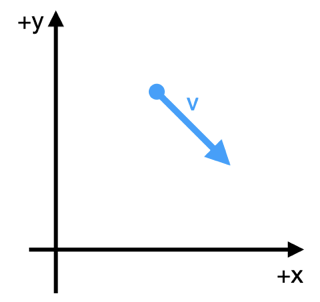
\includegraphics[keepaspectratio,alt={Coordinate System}]{/Users/caballero/repos/teaching/modern-classical-mechanics/images/notes/week4/2d-falling-ball.png}}
\caption{Coordinate System}
\end{figure}

In this coordinate system, the properties of the particle are:

\[\vec{r} = x \hat{x} + y \hat{y} = \langle x, y \rangle\]
\[\vec{v} = v_x \hat{x} + v_y \hat{y} = \langle v_x, v_y \rangle\]
\[\vec{a} = a_x \hat{x} + a_y \hat{y} = \langle a_x, a_y \rangle\]

where \(\hat{x}\) and \(\hat{y}\) are the unit vectors in the \(x\) and
\(y\) directions, respectively. And the magnitude of the velocity vector
is \(|\vec{v}| = \sqrt{v_x^2 + v_y^2}\) as you might imagine.

The free body diagram at the point in time shown above is shown below.
You see the gravitational force pointing directly downward and the drag
force pointing in the opposite direction of the velocity vector. We
continue to apply our coordinate system to the forces.

\begin{figure}
\centering
\pandocbounded{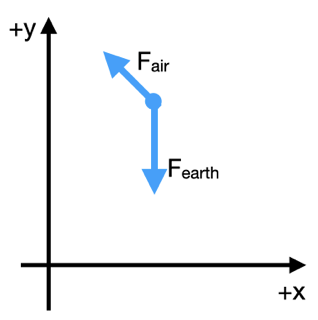
\includegraphics[keepaspectratio,alt={Free Body Diagram}]{/Users/caballero/repos/teaching/modern-classical-mechanics/images/notes/week4/2d-falling-ball-fbd.png}}
\caption{Free Body Diagram}
\end{figure}

\subsubsection{Apply Newton's Second
Law}\label{apply-newtons-second-law}

We now apply Newton's Seccond Law to the particle in the chosen
coordinate system. The forces acting on the particle are the
gravitational force and the drag force.

\[\vec{F}_{net} = \vec{F}_{gravity} + \vec{F}_{drag}\]

How do we apply the coordinate system to the forces? We focus on the
diagram above. We start by writing the sum of the forces. For this, we
take \(F_{gravity,x}\) to be a positive value, \(mg\), where \(g\) is
the magnitude of the acceleration due to gravity.

\[F_{net,x} =  F_{drag,x}\] \[F_{net,y} =  F_{drag,y}-F_{gravity,y}\]

We can now write the forces in terms of the components of the vectors,
and we introduce the acceleration vector,
\(\vec{a} = \langle a_x, a_y \rangle\).

\[m a_x = -D |\vec{v}| v_x\] \[m a_y = -D |\vec{v}| v_y - mg\]

Let's clean this up a little in terms of the components:

\[\ddot{x} = -\frac{D}{m}  \dot{x}\sqrt{\dot{x}^2 + \dot{y}^2}\]
\[\ddot{y} = -\frac{D}{m} \dot{y}\sqrt{\dot{x}^2 + \dot{y}^2} - g\]

We can try to focus on the velocity instead to simplify the equations.
Then we integrate those equations to get the position.

\[\dot{v}_x = -\frac{D}{m}  {v_x}\sqrt{{v_x}^2 + {v_y}^2}\]
\[\dot{v}_y = -\frac{D}{m} {v_y}\sqrt{{v_x}^2 + {v_y}^2} - g\]

Rats! There is no analytical solution to these equations.

These are called
\href{https://math.libretexts.org/Bookshelves/Differential_Equations/Differential_Equations_(Chasnov)/07:_Systems_of_Equations/7.02:_Coupled_First-Order_Equations}{coupled
differential equations} because the equations are linked by the terms
\(\dot{x}\) and \(\dot{y}\). This means that we cannot solve them
independently. We need another approach to solve these equations.

\paragraph{Why can't we solve these
equations?}\label{why-cant-we-solve-these-equations}

We cannot form a solution because they are coupled and non-linear.
Sometimes, we can decouple these equations (as we will see later) and
produce partial differentials of the form:

\[f_1(v_x)dv_x = g_1(t)dt\] \[f_2(v_y)dv_y = g_2(t)dt\]

These lead to independent equations of motion. We can use separation of
variables to try to solve them. This is not possible in all cases, so
functions are still not integrable analytically. But we cannot even form
these partials, so an analytical solution is not possible in this case.

    \subsection{Linear Drag in
Two-Dimensions}\label{linear-drag-in-two-dimensions}

As we saw above, the quadratic drag case is intractable. However, the
linear drag case is analytically solvable. The drag force in 2D can be
written in terms of the velocity vector of the object as:

\[\vec{F}_{lin} = -m \gamma \vec{v}\]

where \(\gamma\) is a proxy for the drag coefficient. The linear drag
force is proportional to the velocity vector.

We have the same set up as before and same FBD.

\begin{figure}
\centering
\pandocbounded{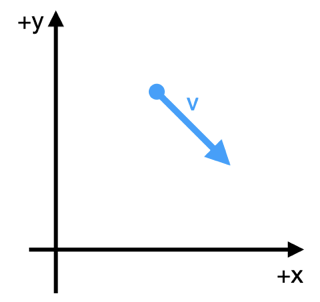
\includegraphics[keepaspectratio,alt={Coordinate System}]{/Users/caballero/repos/teaching/modern-classical-mechanics/images/notes/week4/2d-falling-ball.png}}
\caption{Coordinate System}
\end{figure}

And thus the same coordinate system. The properties of the particle are
the same as above.

\subsubsection{Apply Newton's Second
Law}\label{apply-newtons-second-law}

We now apply Newton's Seccond Law to the particle in the chosen
coordinate system. The forces acting on the particle are the
gravitational force and the drag force.

\[\vec{F}_{net} = \vec{F}_{gravity} + \vec{F}_{lin}\]

Again, the gravitation force magnitude is \(mg\), so we write the forces
in terms of the components of the vectors:

\[F_{net,x} =  F_{lin,x}\] \[F_{net,y} =  F_{lin,y}-F_{gravity,y}\]

In terms of the acceleration vector,
\(\vec{a} = \langle a_x, a_y \rangle\), we have:

\[m a_x = -m \gamma v_x\] \[m a_y = -m \gamma v_y - mg\]

Notice that \(v_x\) and \(v_y\) are the components of the velocity
vector; they can be positive, negative, or zero. We can clean this up in
terms of the velocity components, and we have two linear, uncoupled
differential equations:

\[\dot{v}_x = -\gamma v_x\] \[\dot{v}_y = - \gamma v_y - g\]

\subsubsection{Solve the Equations}\label{solve-the-equations}

We can try to solve these equations by integrating them. We can
integrate the first equation to get the velocity in the \(x\) direction
as a function of time.

\paragraph{\texorpdfstring{Velocity in the \(x\)
direction}{Velocity in the x direction}}\label{velocity-in-the-x-direction}

\[\dot{v}_x = -\gamma v_x\]

We separate the variables and integrate:

\[\frac{dv_x}{v_x} = -\gamma dt\]

We integrate from \(v_{0,x}\) to \(v_x\) and from \(0\) to \(t\):

\[\int_{v_{0,x}}^{v_x} \frac{dv_x}{v_x} = -\gamma \int_{0}^{t} dt\]

\[\ln(v_x) - \ln(v_{0,x}) = -\gamma t\]

\[v_x(t) = v_{0,x} e^{-\gamma t}\]

We see an exponential decay in the velocity in the \(x\) direction.

\paragraph{\texorpdfstring{Velocity in the \(y\)
direction}{Velocity in the y direction}}\label{velocity-in-the-y-direction}

Now we can try to do the same for \(v_y\):

\[\dot{v}_y = -\gamma v_y - g\]

We separate the variables and integrate:

\[\frac{dv_y}{v_y + \frac{g}{\gamma}} = -\gamma dt\]

Note that this integral will be of the form:

\[\int \frac{dx}{x + a} = \ln(x + a) + C\]

Again, we integrate from \(v_{0,y}\) to \(v_y\) and from \(0\) to \(t\):

\[\int_{v_{0,y}}^{v_y} \frac{dv_y}{v_y + \frac{g}{\gamma}} = -\gamma \int_{0}^{t} dt\]

\[\ln(v_y + \frac{g}{\gamma}) - \ln(v_{0,y} + \frac{g}{\gamma}) = -\gamma t\]

\[ln\left(\dfrac{v_y + \frac{g}{\gamma}}{v_{0,y} + \frac{g}{\gamma}}\right) = -\gamma t\]

Next we use exponentiation and do a little algebra to solve for \(v_y\):

\[\left(\dfrac{g}{\gamma} + v_y\right) = \left(\dfrac{g}{\gamma} + v_{0,y}\right) e^{-\gamma t}\]

\[v_y(t) = \dfrac{g}{\gamma}\left(e^{-\gamma t} - 1\right) + v_{0,y} e^{-\gamma t}\]

In the \(y\) direction, the story appears more complex.

\subsubsection{Trajectories}\label{trajectories}

One of the main concepts we will discuss the trajectory of a system. We
borrow that language and idea from projectile motion -- the location of
the particle as a function of time is the trajectory. In this class, we
will consider the word trajectory to mean the evolution of any property
of the system as a function of time. This connects strongly to the
concept of phase space, which we will discuss in the future.

In the prior example, we found the trajectory of the velocity in the
\(x\) and \(y\) directions.

\[v_x(t) = v_{0,x} e^{-\gamma t}\]
\[v_y(t) = \dfrac{g}{\gamma}\left(e^{-\gamma t} - 1\right) + v_{0,y} e^{-\gamma t}\]

We can expound on that work to find the trajectory of the position of
the particle as a function of time. We can integrate the velocity to get
the position.

Those integrals are doable, but they can be a little messy. We won't do
them here, but quote the results consistent with the above equations.

\[x(t) = x_0 + \dfrac{1}{\gamma}v_{0,x}\left(1 - e^{-\gamma t}\right)\]
\[y(t) = y_0 - \dfrac{g}{\gamma}t + \dfrac{1}{\gamma}\left(\dfrac{g}{\gamma} + v_{0,y}\right)\left(1 - e^{-\gamma t}\right)\]

    \subsection{2D Gravitational Bound
System}\label{d-gravitational-bound-system}

Consider a massive object (a large star) and a smaller satellite (a moon
or small planet). We know that
\href{https://en.wikipedia.org/wiki/Newton\%27s_law_of_universal_gravitation}{Newton's
Universal Law of Gravitation} tells us the force between two objects
that interact gravitationally is:

\[F = \dfrac{G m_1 m_2}{r^2}\]

where \(G\) is the gravitational constant, \(m_1\) and \(m_2\) are the
masses of the objects, and \(r\) is the distance between the objects.

But we need to be more clear about the forces and the vector
relationships. Consider the figure below with the massive object at the
origin and the satellite at some distance \(r\) from the origin. What is
the vector \(\vec{r}\) that describes the location of the satellite?

\begin{figure}
\centering
\pandocbounded{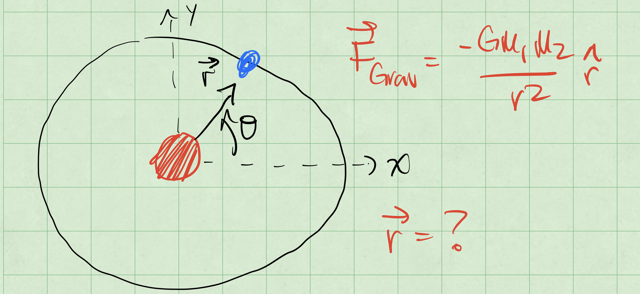
\includegraphics[keepaspectratio,alt={Gravitational Bound System}]{/Users/caballero/repos/teaching/modern-classical-mechanics/images/notes/week4/grav_01.png}}
\caption{Gravitational Bound System}
\end{figure}

If we move the sun from the origin a little, we can start to see what
\(\vec{r}\) is. The vector \(\vec{r}\) is the vector from the sun to the
satellite. See the figure below to see the sketch.

\begin{figure}
\centering
\pandocbounded{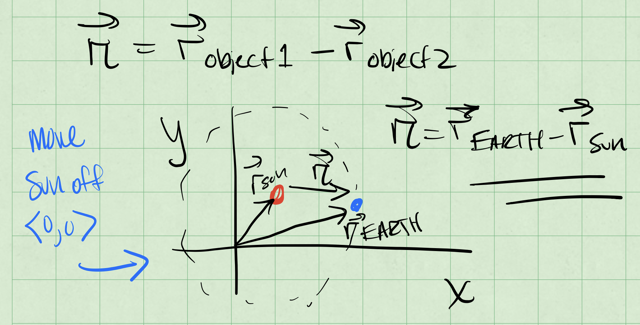
\includegraphics[keepaspectratio,alt={Gravitational Bound System}]{/Users/caballero/repos/teaching/modern-classical-mechanics/images/notes/week4/grav_02.png}}
\caption{Gravitational Bound System}
\end{figure}

So if the location of the sun is \(\vec{r}_{sun}\) and the Earth is
\(\vec{r}_{earth}\), then the vector \(\vec{r}\) is:

\[\vec{r} = \vec{r}_{earth} - \vec{r}_{sun}\]

Let's return to the simplified model with the sun at the origin, and
consider the earth at some distance \(r\) from the origin. The force on
the earth is:

\[\vec{F}_{grav} = -G \dfrac{M_{sun} M_{earth}}{|\vec{r}|^3} \vec{r}\]

where \(M_{sun} = 2\times10^{30} \mathrm{kg}\) is the mass of the sun
and \(M_{earth} = 6 \times 10^{24} \mathrm{kg}\) is the mass of the
earth.

\subsubsection{Define the Coordinate
System}\label{define-the-coordinate-system}

In the figure below, we show the earth at some distance \(r\) from the
origin at an angle \(\phi\) from the \(x\)-axis. This distance is about
\(1.5 \times 10^{11}\;\mathrm{m}\) or \(1\;\mathrm{A.U.}\)
(\href{https://en.wikipedia.org/wiki/Astronomical_unit}{astronomical
unit}). While not entirely obvious, the scale of these numbers allow us
to assume the Sun is at the origin, and doesn't move. Although this is
not a good assumption for the real solar system, the sun orbits the
\href{https://en.wikipedia.org/wiki/Barycenter}{barycenter} of the solar
system, which is about 1 solar radii from the center of the sun.

\begin{figure}
\centering
\pandocbounded{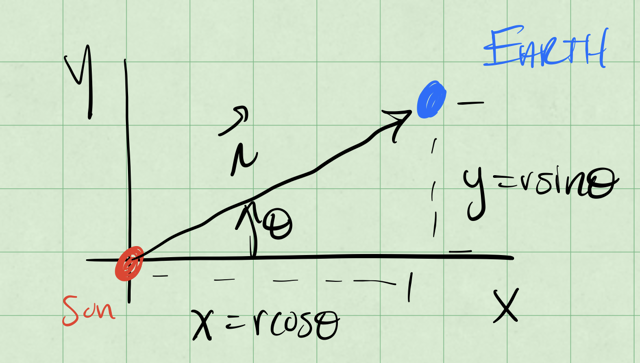
\includegraphics[keepaspectratio,alt={Gravitational Bound System}]{/Users/caballero/repos/teaching/modern-classical-mechanics/images/notes/week4/grav_03.png}}
\caption{Gravitational Bound System}
\end{figure}

Let's use the standard \(x\) and \(y\) axes to write the equations of
motion. We can apply Newton's Second Law to the earth in the chosen
coordinate system.

\[\vec{F}_{net} = \vec{F}_{gravity} = m\vec{a} = m\langle a_x, a_y \rangle\]

So that the forces in the \(x\) and \(y\) directions are:

\[F_x = -G \dfrac{M_{sun} M_{earth}x}{(x+2+y^2)^{3/2}} \qquad F_y = -G \dfrac{M_{sun} M_{earth}y}{(x+2+y^2)^{3/2}}\]

and thus the acceleration of the Earth in the \(x\) and \(y\) directions
are:

\[a_x = -G \dfrac{M_{sun} x}{(x+2+y^2)^{3/2}} \qquad a_y = -G \dfrac{M_{sun} y}{(x+2+y^2)^{3/2}}\]

This gives us a set of coupled differential equations.

\[\ddot{x} = -G \dfrac{M_{sun} x}{(x+2+y^2)^{3/2}} \qquad \ddot{y} = -G \dfrac{M_{sun} y}{(x+2+y^2)^{3/2}}\]

\subsubsection{How do we then get the
trajectories?}\label{how-do-we-then-get-the-trajectories}

We can't solve these equations without more information. We need to know
the initial conditions of the system (the initial position and velocity
of the Earth). We can then integrate these equations to get the position
of the Earth as a function of time.

We have three potential ways to solve these EOMs:

\begin{enumerate}
\def\labelenumi{\arabic{enumi})}
\tightlist
\item
  Direct Integration: We can integrate the equations of motion directly.
  This is possible in some cases where the equations are simple enough;
  think about the falling ball without air resistance, or the linear 1D
  drag case.
\item
  Decouple and Solve: We try to solve the coupled differential equations
  by decoupling them. This is possible in some cases, but not all. We
  can frequently decouple the equations by writing them in terms of the
  velocity, or by making a change of position variables.
\item
  Numerical Integration: We use numerical methods to predict the motion
  in small time steps. This is the most common method for solving
  complex systems.
\end{enumerate}

    

    \subsection{The Simple Harmonic Oscillator
(SHO)}\label{the-simple-harmonic-oscillator-sho}

In 1D, the simple harmonic oscillator is a system where the force is
proportional to the displacement from the equilibrium position. The
force is given by:

\[F = -ks\]

where \(k\) is the spring constant and \(s\) is the displacement from
the equilibrium position, \(x-L_0\). The quantity \(L_0\) is the relaxed
length of the spring. The figure below shows the typical horizontal
spring system.

\begin{figure}
\centering
\pandocbounded{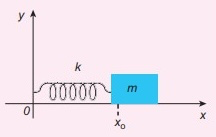
\includegraphics[keepaspectratio,alt={SHO}]{/Users/caballero/repos/teaching/modern-classical-mechanics/images/notes/week3/sho_horizontal.png}}
\caption{SHO}
\end{figure}

We can typically choose to measure the displacement from the equilibrium
position, and write the force instead as:

\[F = m a_x = m \dot{v}_x  = m\ddot{x} = -kx\]

So the equation of motion that we will try to solve is:

\[\ddot{x} = -\dfrac{k}{m}x\]

\subsubsection{How do we solve this?}\label{how-do-we-solve-this}

\[\dfrac{d^2x}{dt^2} = -\dfrac{k}{m}x = - \omega^2 x\]

where \(\omega = \sqrt{\dfrac{k}{m}}\) is the natural oscillation
frequency of the system.

It might seem strange, but let's try the following potential solution to
the differential equation:

\[x(t) = C e^{i\omega t}\]

where \(C\) is a constant. We can take the second derivative of \(x(t)\)
with respect to time to see if it satisfies the differential equation.

\[\dot{x}(t) = i\omega C e^{i\omega t}\]
\[\ddot{x}(t) = -\omega^2 C e^{i\omega t} = -\omega^2 x(t)\]

This is a solution to the differential equation as long as \(C\) is a
constant, but it's a complex one (\(C=a+ib\)). We can also write the
solution in terms of the cosine and sine functions because the
exponential function can be written in terms of these functions.

\[e^{i\omega t} = \cos(\omega t) + i\sin(\omega t)\]

Thus, another general solution to this EOM that we can write is:

\[x(t) = A \cos(\omega t) + B \sin(\omega t)\]

where \(A\) and \(B\) are constants that depend on the initial
conditions of the system. Let's see how that works:

\[\dot{x}(t) = -A \omega \sin(\omega t) + B \omega \cos(\omega t)\]
\[\ddot{x}(t) = -A \omega^2 \cos(\omega t) - B \omega^2 \sin(\omega t) = -\omega^2 x(t)\]

Another form that works is:

\[x(t) = D \cos(\omega t + \phi)\]

where \(D\) is the amplitude of the oscillation and \(\phi\) is the
phase of the oscillation. Let's check that again:

\[\dot{x}(t) = -D \omega \sin(\omega t + \phi)\]
\[\ddot{x}(t) = -D \omega^2 \cos(\omega t + \phi) = -\omega^2 x(t)\]

So we have several forms of the general solution to the simple harmonic
oscillator. We can use these solutions to understand the behavior of the
system. We can also use these solutions to understand the behavior of
more complex systems that can be approximated by the simple harmonic
oscillator.

One critical aspect of these solutions is that they have 2 free
parameters, \(A\) and \(B\), or \(D\) and \(\phi\). These parameters are
determined by the initial conditions of the system. \textbf{There are N
free parameters in the general solution to an Nth order differential
equation.}

    


    % Add a bibliography block to the postdoc
    
    
    
\end{document}
